\chapter{Funciones}
\label{funcchap}

En el contexto de la programación, una {\bf función}
es usualmente una secuencia de sentencias con nombre
que realizan una computación. En Perl, las funciones
son usualmente llamadas {\bf subrutinas} y los dos términos
(por ahora) pueden considerarse  más o menos equivalente. Cuando defines
una función, especificas el nombre y la secuencia de sentencias.
Después, cuando quieras realizar la computación, puedes 
``invocar`` la función por el nombre y esto ejecutará la secuencia
de sentencias dentro de la definición de la función.
\index{function}

Perl viene como muchas funciones integradas que son muy útiles.
Ya has visto algunas de ellas: por ejemplo, {\tt say} es una función 
integrada, y veremos más en el curso de este libro. Y si Perl no tiene
una función que hace lo que deseas hacer, tú puedes construirla. Esto
te enseña lo básico de las funciones y cómo construir una.

\section{Llamadas de Funciones}
\label{functionchap}
\index{function!call}

Ya hemos visto algunos ejemplos de {\bf llamadas de funciones}:

\begin{verbatim}
> say 42;
42
\end{verbatim}
%
El nombre de la función es {\tt say}. La expresión que sigue el
nombre de la función se llama el {\bf argumento} de la función.
La función {\tt say} causa que el argumento se ha mostrado en 
la pantalla. Si necesitas pasar varios argumentos a la función, 
solo separa los argumentos con comas:

\begin{verbatim}
> say "La respuesta a la pregunta absoluta es ", 42;
La respuesta a la pregunta absoluta es 42
\end{verbatim}
%

Muchos lenguajes de programación requieren que los argumentos de
la función se encuentren dentro de paréntesis. Esto no es requerido
(y usualmente no recomendado) en Perl~6 para la mayoría de 
las funciones integradas (excepto cuando se necesita para 
precedencia), pero si usas paréntesis, deberías evitar insertar 
espacios entre el nombre de la función y el paréntesis izquierdo,
Por ejemplo, la función {\tt round} usualmente toma dos argumentos:
el valor a ser redondeado y la unidad o escala.
Puedes invocarla en cualquiera de las siguientes formas:

\begin{verbatim}
> round 42.45, 1;
42
> round 42.45, .1;
42.5
> round(42.45, .1);      # Pero no: round (42.45, .1);
42.5
> round( 42.45, .1);     # Espacio *después* del paréntesis izq. es OK 
42.5
\end{verbatim}
\index{parentheses!argument in}

Los programadores de Perl con experiencia prefieren omitir los 
paréntesis cuando ellos pueden. Esto hace posible encadenar varias 
funciones con una sintaxis más limpia. Considera por ejemplo
la diferencia entre estas dos llamadas:

\begin{verbatim}
> say round 42.45, 1;
42
> say(round(42.45, 1));
42
\end{verbatim}

La segunda sentencia dice explícitamente lo que está pasando,
pero la acumulación de paréntesis actualmente no hace las cosas
muy claras. Por el contrario, la primera sentencia puede ser
considerada como una línea de tuberías que se puede leer de derecha 
a izquierda: la última función a la derecha, {\tt round}, toma dos
argumentos, {\tt 42.45, 1}, y el valor producido por {\tt round}
es pasado como un argumento a {\tt say}.

Es muy común decir que una función ``toma`` uno o varios
argumentos y ``devuelve`` un resultado. El resultado es también
llamado el {\bf valor de retorno}.
\index{argument}
\index{return!value}

Perl provee varias funciones que convierten valores de un
tipo a otro. Cuando se invocan con un solo argumento,
la función {\tt round} toma cualquier valor y lo convierte
en un número entero, o por el contrario se queja:
\index{conversion!type}
\index{type!conversion}
\index{round function}
\index{function!round}

\begin{verbatim}
> round 42.3;
42
> round "yes"
Cannot convert string to number: base-10 number must begin with valid 
digits or '.' in '<HERE>yes' (indicated by <HERE>)
  in block <unit> at <unknown file> line 1
\end{verbatim}

%
Nota que, en Perl~6, muchas funciones integradas pueden también
usar la sintaxis de la \emph{llamada de método} con la así 
llamada notación de punto. Las siguientes sentencias muestran el 
mismo resultado:
\index{invocation!method}
\index{method invocation}
\begin{verbatim}
> round 42.7;    # Sintaxis de la llamada de función
43
> 42.7.round;    # Sintaxis de la llamada de método
43
\end{verbatim}
%
La función {\tt round} puede redondear valores racionales
y valores coma flotante. Hay un método {\tt Int} que también
convierte valores numéricos no enteros en enteros, pero
no redondea; corta la parte fraccional:
\index{Int method}
\index{method!Int}

\begin{verbatim}
> round 42.7
43
> 42.7.Int
42
\end{verbatim}

Volveremos a los métodos en la siguiente sección.

La función integrada {\tt Rat} convierte números
enteros y cadenas de texto en números racionales (si es posible):
\index{Rat function}
\index{function!Rat}

\begin{verbatim}
> say 4.Rat;
4
> say 4.Rat.WHAT;
(Rat)
> say Rat(4).WHAT;
(Rat)
> say Rat(4).nude;
(4 1)
> say Rat('3.14159');
3.14159
> say Rat('3.14159').nude
(314159 100000)
\end{verbatim}
%
(Como podrás recordar de la Sección~\ref{values_and_types}, 
el método \verb'nude' muestra el \emph{nu}merador y  
\emph{de}nominador de un número racional.)

Finalmente, {\tt Str} convierte su argumento a una cadena de texto:
\index{Str function}
\index{function!Str}

\begin{verbatim}
> say 42.Str.WHAT
(Str)
> say Str(42).WHAT;
(Str)
\end{verbatim}

\index{coercion}
\index{type!coercion}
Nota que estas funciones de conversión de tipo no necesitan ser
invocadas explícitamente, dado que Perl intentará hacer lo correcto
en muchos de los casos. Por ejemplo, si tienes una cadena de texto
que se parece a un número entero, Perl \emph{coaccionará} la cadena 
de texto en un entero para ti si tratas de aplicarle una operación 
aritmética:

\begin{verbatim}
> say "21" * "2";
42
\end{verbatim}

Igualmente, los enteros serán coaccionados en cadenas de texto
si aplicas el operador de la concatenación de cadena de texto
sobre ellos:

\begin{verbatim}
> say 4 ~ 2;
42
> say (4 ~ 2).WHAT;
(Str)
\end{verbatim}

La coacción puede hasta pasar dos veces dentro de la misma expresión
si necesario:

\begin{verbatim}
> say (4 ~ 1) + 1;
42
> say ((4 ~ 1) + 1).WHAT;
(Int)
\end{verbatim}

\section{Funciones y Métodos}
\index{function}
\index{method}

Un método es similar a una función---toma argumentos y 
devuelve un valor---pero la sintaxis de llamada es
diferente. Con una función, especificas el nombre de la función
seguido de sus argumentos. Un método, por el contrario, usa 
la notación de punto: tu especificas el nombre del objecto
sobre el cual el método es invocado, seguido por un punto y
el nombre del método (y posiblemente argumentos adicionales).

% 
Una llamada de método es usualmente conocida como una 
{\bf invocación} \index{invocation}. Las diferencias más
profundas entre funciones y métodos se volverá aparente 
más adelante, cuando estudiemos la programación orientada
a objetos (en el Capítulo~\ref{objects}).
\index{invocation!method}
\index{method invocation}

Por el tiempo presente, podemos consider que la diferencia
es esencialmente un asunto de una sintaxis diferente de 
llamada cuando se usan las funciones integradas de Perl. La mayoría
de las funciones integradas en Perl aceptan la sintaxis de la llamada
de función y la sintaxis de la invocación de método. Por ejemplo,
las siguientes sentencias son equivalentes:

\begin{verbatim}
> say 42;              # sintaxis de la llamada de función
42
> 42.say;              # sintaxis de la invocación de método
42
\end{verbatim}
%

También puedes encadenar subrutinas con ambas formas
sintácticas:

\begin{verbatim}
> 42.WHAT.say;         # sintaxis de método
(Int)
> say WHAT 42;         # sintaxis de función
(Int)
> say 42.WHAT;         # sintaxis mixta
(Int)
\end{verbatim}
%

Depende de ti cuál de las formas prefieres usar, pero
usaremos ambas formas, aún solo sea para acostumbrarnos
a ambas.

\section{Funciones Matemáticas}
\index{math function}
\index{function!math}

Perl provee muchas de las funciones matemáticas familiares.

Para algunas funcionesno tan comunes, podría necesitar un
módulo especializado tal com \verb'Math::Matrix' o
\verb'Math::Trig'. Un {\bf módulo} es un archivo de texto 
que contiene una colección de funciones que están relacionadas.
\index{module}

Antes de que usemos las funciones en un módulo, tenemos que importarlo
la sentencia {\bf use}:

\begin{verbatim}
use Math::Trig;
\end{verbatim}
%
Esta sentencia importará un número de funciones que serás capaz de usar
como si tu las hubieses definido en el archivo de código principal,
por ejemplo \verb|grad2rad| convierte un valor angular desde grados
a radianes o \verb|rad2grad| que hace la conversión opuesta.

Para la mayoría de funciones matemáticas comunes, sin embargo, no necesitas
tener ningún módulo \verb|matemático|, dado que dichas funciones
ya están incluidas en núcleo del lenguaje:

\begin{verbatim}
> my $nivel-ruido = 5.5;
5.5
> my $nivel-señal = 125.6;
125.6
> my $decibelios = 10 * log10 $nivel-señal / $nivel-ruido;
13.5862694990693
\end{verbatim}
%
\index{log10 function}
\index{function!log10}
El primer ejemplo usa \verb"log10" (logaritmo común)
para computar la razón de señal y ruido en decibelios
(asumiendo que \verb|nivel-señal| y \verb|nivel-ruido| sean 
definidos en las propias unidades). Perl también provee una 
función {\tt log}, la cual, cuando recibe un argumento,
computa el logaritmo en base {\tt e} del argumento y,
cuando recibe dos argumentos, computa el logaritmo del primer
argumento en base del segundo argumento:

\begin{verbatim}
> say e;                 # e es predefinada como la constante de Euler
2.71828182845905
> my $val = e ** e;
15.1542622414793
> say log $val;          # logaritmo natural
2.71828182845905
> say log $val, e;       # logaritmo en base e o logaritmo natural
2.71828182845905
> say log 1024, 2;       # logaritmo binario o logaritmo en base 2
10
\end{verbatim}
%
\index{log function}
\index{function!log}

Perl también provee muchas de las funciones trigonométricas
comunes:

\begin{verbatim}
> my $radianes = 0.7;
0.7
> my $altura = sin $radianes;
0.644217687237691
\end{verbatim}

\index{sin function}
\index{radian}
\index{trigonometric function}
\index{function!trigonometric}
Este ejemplo encuentra el seno de \verb|$radianes|. El 
nombre de la variable es una pista a que el {\tt sin} y 
otras funciones trigonométricas ({\tt cos}, {\tt tan}, etc.) toman
argumentos en radianes. Para convertir de grados a radianes, puedes
usar la función \verb'deg2rad' del  módulo \verb|Math::Trig|, o
simplemente divide por 180 y multiplica por $\pi$:

\begin{verbatim}
> my $grados = 45;
45
> my $radianes = $grados / 180.0 * pi;    # pi, constante predefinida 
0.785398163397448
> say sin $radianes;       # debería ser la raíz cuadrada de 2 divida por 2
0.707106781186547
\end{verbatim}
%
La expresión {\tt pi} es una constante predefinida de una
aproximación de $\pi$, precisa alrededor de 14 dígitos:
\index{pi}

Si sabes trigonometría, puedes verificar el resultado anterior
al compararlo con la raíz cuadrada de 2 dividida por 2:
\index{sqrt function}
\index{function!sqrt}

\begin{verbatim}
> say sqrt(2) / 2;
0.707106781186548
\end{verbatim}
%

\section{Composición}
\index{composition}

Hasta ahora, hemos discutidos los elementos de un programa---variables,
expresiones, y sentencias---aisladamente, sin discutir sobre
cómo combinarlos.

Una de las características más útiles de los lenguajes de programación
es su habilidad de tomar pequeños componentes y {\bf componer} estos
componentes, i.e.,
combinarlos de tal manera que el resultado de uno es la entrada
de otro. Por ejemplo, el argumento de una función  puede ser cualquier
tipo de expresión, incluyendo operadores aritméticos:

\begin{verbatim}
> my $grados = 45;
45
> my $altura = sin($grados / 360.0 * 2 * pi);
0.707106781186547
\end{verbatim}
%
Aquí, hemos usados paréntesis para el argumento de la función
{\tt sin} para clarificar que todas las operaciones aritméticas
sean completadas antes que la función {\tt sin} sea actualmente
llamada, para que así use el resultado de estas operaciones 
como su argumento.

Puedes componer llamadas de funciones:

\begin{verbatim}
> my $x = 10;
10
>  $x = exp log($x+1)
11
\end{verbatim}
%
Casi en cualquier lado que puedes poner un valor, puedes poner
una expresión arbitraria, con una excepción: el lado izquierdo 
de la sentencia de asignación tiene que ser el nombre de una
variable, posiblemente con su declaración. Casi cualquier otra expresión
en el lado izquierdo es un error sintáctico \footnote{Veremos esta rara
excepción a esta regla más tarde}:


\begin{verbatim}
> my $horas = 1;
1
> my $minutos = 0;
0
> $minutos = $horas * 60;        # correcto 
60
> $horas * 60 = $minutos;        # incorrecto!!
Cannot modify an immutable Int
  in block <unit> at <unknown file> line 1
\end{verbatim}
%
\index{syntax error}


\section{Agregar Nuevas Funciones (o Subrutinas)}

\index{subroutine}
Hasta ahora, hemos solo usado las funciones que vienen con Perl,
pero también es posible agregar nuevas funciones. En Perl, las 
funciones definidas por el usuario son usualmente conocidas 
como subrutinas, pero podrías eligir cualquiera de las dos
palabras. 

Una {\bf definición de función} comienza con la palabra clave 
{\tt sub} (abreviación de subrutina) y especifica el nombre de una
nueva subrutina y la secuencia de sentencias que serán ejecutadas
cuando función es llamada.
\index{function}
\index{function!definition}
\index{definition!function}
\index{sub}

Este es un ejemplo de una subrutina que cita el famoso discurso
"I Have a Dream" de Martin Luther King en el Lincoln Memorial en
Washington (1963):

\begin{verbatim}
sub imprimir-discurso() {
    say "Let freedom ring from the prodigious hilltops of New Hampshire.";
    say "Let freedom ring from the mighty mountains of New York.";
}
\end{verbatim}
%
{\tt sub} es la palabra clave que indica que esto es una definición 
de subrutina. El nombre de la función es \verb|imprimir-discurso|.
Las reglas para los nombres de subrutinas son las mismas reglas 
para los nombres de variables: letras, números, y guiones bajos son
legales, al igual que un guión o un apóstrofo entre letras, pero
el primer carácter debe ser una letra o un guion bajo. No deberías
usar una palabra clave usada por el lenguaje (tales como {\tt if} 
o {\tt while}) como el nombre de una función (en algunos casos, podría
actualmente funcionar pero sería algo confuso, por lo menos 
para el lector humano).
\index{sub!keyword}
\index{keyword!sub}
\index{argument}

Los paréntesis vacíos después del nombre indican que esta función 
no toma ningún argumento. En tal caso los argumentos son opcionales,
pero son requeridos cuando los parámetros necesitan ser definidos para
la subrutina.
\index{parentheses!empty}
\index{header}
\index{body}

\index{indentation}
La primera línea de la definición de una subrutina es algunos
veces llamada la {\bf cabecera}; el resto es conocido como el
{\bf cuerpo} de la subrutina. El cuerpo tiene que ser un bloque de
código colocado entre llaves y puede contener una cantidad
indefinida de sentencias. Aunque no existe una regla que lo requiera,
es buena práctica (y muy recomendada) la indentación de las sentencias
en el cuerpo con varios espacios delanteros, debido a que facilita
descifrar visualmente donde el cuerpo de la función inicia y termina.
\index{curly bracket}
\index{curly brace}
\index{bracket!curly}

Ten presente que no puedes utilizar la sintaxis de invocación de método
con las subrutinas (tal como \verb|imprimir-discurso|) que escribas: 
debes llamarlas con la sintaxis de llamada de función.
\index{method!invocation}
\index{function!call}
\index{invocation!method}
\index{method invocation}

Las cadenas de texto en las sentencias de impresión están rodeadas
por comillas inglesas. En este caso específico, las comillas simples
se podrían haber usado para obtener el mismo resultado, pero
hay otros casos donde los dos tipos de comillas no harían lo mismo,
así que tendrás que elegir una de las dos dependiendo de las 
circunstancias.
\index{double quote}
\index{quote!double}
\index{single quote}
\index{quote!single}

Muchas personas usan las comillas inglesas en los casos
donde una comilla simple (la cual también es un apóstrofo)
aparece en una cadena de texto:
\index{apostrophe}
\begin{verbatim}
say "And so we've come here today to dramatize a shameful condition.";
\end{verbatim}
%
De igual manera, podrías utilizar comillas simples 
cuando las comillas inglesas aparecen en una cadena de texto:
\begin{verbatim}
say 'America has given the Negro people a bad check, 
     a check which has come back marked "insufficient funds."';
\end{verbatim}
%
Sin embargo, existe una diferencia más importante entre las 
comillas simples y las comillas inglesas: las comillas inglesas
permiten la interpolación de variables, lo cual no es posible
con el uso de comillas simples. La interpolación de variables
se refiere a que si el nombre de una variable aparece dentro
de una cadena de texto rodeada por comillas inglesas, dicho 
nombre será reemplazado por el valor de la variable; dentro una 
cadena de texto rodeada por comillas simples, el nombre de la 
variable aparecerá literalmente.
Por ejemplo:
%
\begin{verbatim}
my $var = 12;
say "La edad del niño es $var.";         # -> La edad del niño es 12.
say 'La edad de la niña es $var.';       # -> La edad de la niña es $var.
\end{verbatim}
\index{interpolation}
\index{variable!interpolation}
%
La edad de la niña no se muestra porque se quiera mantener un
secreto. En la primera cadena de texto, \verb|$var| es 
simplemente reemplazada dentro de la cadena por su valor, 12, porque
la cadena de texto está rodeada con comillas inglesas; en la segunda
cadena de texto, \verb|$var| no es reemplazada por su valor porque las 
comillas simples están supuestas a proveer un citado más literal. 
Existen otros tipos de citados que ofrecen un mayor control sobre la
manera en que las variables y los caracteres especiales son mostrados 
en la salida, pero las comillas simples y las comillas inglesas
son las más útiles.

La sintaxis para llamar una nueva subrutina es la misma usada
para llamar las funciones integradas:

\begin{verbatim}
> imprimir-discurso();
Let freedom ring from the prodigious hilltops of New Hampshire.
Let freedom ring from the mighty mountains of New York.
\end{verbatim}
%

No obstante, no puedes utilizar la sintaxis de invocación de método
con tales subrutinas. Más tarde veremos en este libro (ve
Capítulo~\ref{objects}) cómo crear métodos. Por el tiempo presente,
permaneceremos con la sintaxis de llamada de función.
\index{invocation!method}
\index{method invocation}

Una vez que has definido una subrutina, puedes usarla dentro
de otra subrutina. Por ejemplo, para repetir el fragmento anterior
del discurso de King, podríamos escribir una subrutina llamada 
\verb|repetir-discurso|:

\begin{verbatim}
sub repetir-discurso() {
    imprimir-discurso();
    imprimir-discurso();
}
\end{verbatim}
%
Y después llamar \verb|repetir-discurso|:

\begin{verbatim}
> repetir-discurso();
Let freedom ring from the prodigious hilltops of New Hampshire.
Let freedom ring from the mighty mountains of New York.
Let freedom ring from the prodigious hilltops of New Hampshire.
Let freedom ring from the mighty mountains of New York.
\end{verbatim}
%
No obstante, no es así como prosigue el discurso.


\section{Definiciones y Usos}
\index{function!definition}

Juntando los fragmentos de código de la sección anterior, el
programa entero luce así:

\begin{verbatim}
sub imprimir-discurso () {
    say "let freedom ring from the prodigious hilltops of New Hampshire.";
    say "Let freedom ring from the mighty mountains of New York.";
}
sub repetir-discurso () {
    imprimir-discurso();
    imprimir-discurso();
}
repetir-discurso();
\end{verbatim}
%
Este programa contiene dos definiciones de subrutinas: \verb|imprimir-discurso|
y \verb|repetir-discurso|. Las definiciones de funciones pueden ser ejecutadas
como otras sentencias, pero el efecto es crear la función. Las sentencias
dentro de la función no son ejecutadas hasta que la función es llamada, y
la definición de la función no genera ninguna salida.

No necesitas crear una subrutina antes de ejecutarla,
la definición de la función puede venir después de la llamada:

\begin{verbatim}
repetir-discurso;
sub repetir-discurso() {
    imprimir-discurso;
    imprimir-discurso;
}
sub imprimir-discurso() {
    # ...
}
\end{verbatim}


\section{Flujo de Ejecución}
\index{flow of execution}

Para asegura, por ejemplo, que una variable está definida (i.e. poblada)
antes de sus uso, necesitas saber el orden en el que las sentencias se
ejecutan. Dicho orden es conocido como el {\bf flujo de ejecución}.

La ejecución siempre con la primera sentencia del programa (bueno, {\bf casi}
siempre, pero digamos siempre por el tiempo presente). Las sentencias se
ejecutan una por una, de arriba hacia abajo.

Las definiciones de subrutinas no cambian el flujo de ejecución del 
programa, pero debes recordar que las sentencias dentro de una función
no son ejecutadas hasta que la función es llamada.

Una llamada de función es como un desvío en el flujo de ejecución. En vez
de continuar con la siguiente sentencia, el flujo salta al cuerpo de la función,
ejecuta las sentencias ahí dentro, y regresa para continuar donde se
quedó.

Esto suena simple hasta que recuerdas que una función puede llamar otra función.
Mientra se encuentra dentro de una función, el programa podría ejecutar las
sentencias en otra función. ¡Después, mientra se encuentra en dicha función,
el programa podría aún ejecutar otra función!

Afortunadamente, Perl es lo suficientemente bueno para rastrear dónde 
se encuentra, así que cada vez una función se completa, el programa continúa 
donde se quedó en el programa que lo llamó. Cuando llega al final del programa,
entonces termina.

En resumen, cuando leas un programa, no siempre quieras leerlo de 
arriba hacia abajo. Algunas hace más sentido si sigues el flujo de
ejecución.

\section{Parámetros y Argumentos}
\label{parameters}
\index{parameter}
\index{function!parameter}
\index{argument}
\index{function!argument}

Algunas de la funciones que hemos requieren argumentos. Por ejemplo,
cuando llamas a {\tt sin} tu le pasas un número como argumento. Algunas
funciones toman más de un argumento: por ejemplo, la función {\tt round}
que vimos al principio de este capítulo tomó dos, el número a ser redondeado
y la escala (aunque la función {\tt round} puede aceptar un solo 
argumento. En dicho caso, el valor de la escala por defecto es 1).
 
Dentro de la subrutina, los argumentos son asignados a variables llamadas 
{\bf parámetros}. Aquí está la definición de una subrutina que toma un 
solo argumento:
\index{parentheses!parameters in}

\begin{verbatim}
sub doble-impresión($valor) {
    say $valor;
    say $valor
}
\end{verbatim}
%
Esta subrutina asigna el argumento al parámetro llamado
\verb|$valor|. Otra manera común de interpretarlo es decir que
la subrutina ata el parámetro definido en su cabecera al argumento
con el cual es llamada. Cuando la subrutina anterior es llamada, 
imprimer el contenido del parámetro (cualquier cosa que sea) dos
veces.

Esta función funciona con cualquier argumento que pueda ser
imprimido:

\begin{verbatim}
> doble-impresión("Let freedom ring")
Let freedom ring
Let freedom ring
> doble-impresión(42)
42
42
> doble-impresión(pi)
3.14159265358979
3.14159265358979
\end{verbatim}
%
Las mismas reglas de composición que aplican a la funciones integradas 
también aplican a las funciones definidas por el programador, así que podemos
cualquier tipo de expresión como un argumento para \verb|doble-impresión|:
\index{composition}
\index{programmer-defined function}
\index{function!programmer defined}

\begin{verbatim}
> doble-impresión('Let freedom ring! ' x 2)
Let freedom ring! Let freedom ring! 
Let freedom ring! Let freedom ring! 
> doble-impresión(cos pi)
-1
-1
\end{verbatim}
%
El argumento es evaluado antes que la función sea llamada, 
así que en los ejemplos las expresiones \verb"'Let freedom ring! ' x 2" 
y {\tt cos pi} son evaluadas una sola vez.
\index{argument}

También puedes usar una variable como argumento:

\begin{verbatim}
> my $declaración = 'When in the Course of human events, ...'
> doble-impresión($declaración)
When in the Course of human events, ...
When in the Course of human events, ...
\end{verbatim}
%
El nombre de la variable que pasamos como un argumento (\verb|$declaración|)
no tiene nada que ver con el nombre del parámetro (\verb|$valor|). No
importa cual sea el nombre de la variable cuando fue llamada;
aquí, dentro de \verb|doble-impresión|, llamamos al parámetro 
\verb|$valor| sin importar el nombre o contenido del argumento que se
pasó a la subrutina.


\section{Las Variables y los Parámetros Son Locales}
\index{local variable}
\index{variable!local}
\index{scope}
\index{my}
\index{lexical scope}
\label{localvar}

Cuando creas una variable dentro de una subrutina con 
la palabra clave {\tt my}, dicha variable es entonces 
local, o más precisamente, la variable está en un {\tt ámbito
lexical} con respecto al bloque de la función. Esto significa
que la variable solo existe dentro de la función. Por ejemplo:
\index{parentheses!parameters in}

\begin{verbatim}
sub doble_concat($parte1, $parte2) {
    my $concatenación = $parte1 ~ $parte2;
    doble-impresión($concatenación)
}
\end{verbatim}
%
Esta función toma dos argumetos, los concatena, e imprime
el resultado dos veces. Este es un ejemplo que la usa:
\index{concatenation}

\begin{verbatim}
> my $inicio = 'Let freedom ring from ';
> my $final = 'the mighty mountains of New York.';
> doble_concat($inicio, $final);
Let freedom ring from the mighty mountains of New York.
Let freedom ring from the mighty mountains of New York.
\end{verbatim}
%
Cuando \verb|doble-concat| terminar, la variable \verb|$concatenación|
es destruida. Si intentamos imprimirla, obtenemos una excepción:
\index{Variable ... is not declared}
\index{exception!not declared}

\begin{verbatim}
> say $concatenación;
===SORRY!=== Error while compiling <unknown file>
Variable '$concatenación' is not declared
at <unknown file>:1
------> say <HERE>$concatenación;
\end{verbatim}
%
Los parámetros también están en un ámbito lexical
en la subrutina. Por ejemplo, fuera de \verb|doble-impresión|, 
no existe tal como \verb|$valor|.
\index{parameter}
\index{scope}


\section{Diagramas de Pila}
\label{stackdiagram}
\index{stack diagram}
\index{function!frame}
\index{frame}

Para rastrear cual de las variables puede ser usada, es algunas veces
muy útil dibujar un {\bf diagrama de pila}. Al igual que los diagramas de
estado, los diagramas de pila muestran el valor de cada variable, pero
también muestran la función a la cual cada variable pertenece.
\index{stack diagram}
\index{diagram!stack}

Cada función se representa gráficamente por un {\bf marco}. Un marco
es una cuadro con el nombre de la función al lado y los parámetros y
las variables de la función dentro. El diagrama de pila 
para el ejemplo anterior se muestra en la Figura~\ref{fig.stack}.

\begin{figure}
\centerline
{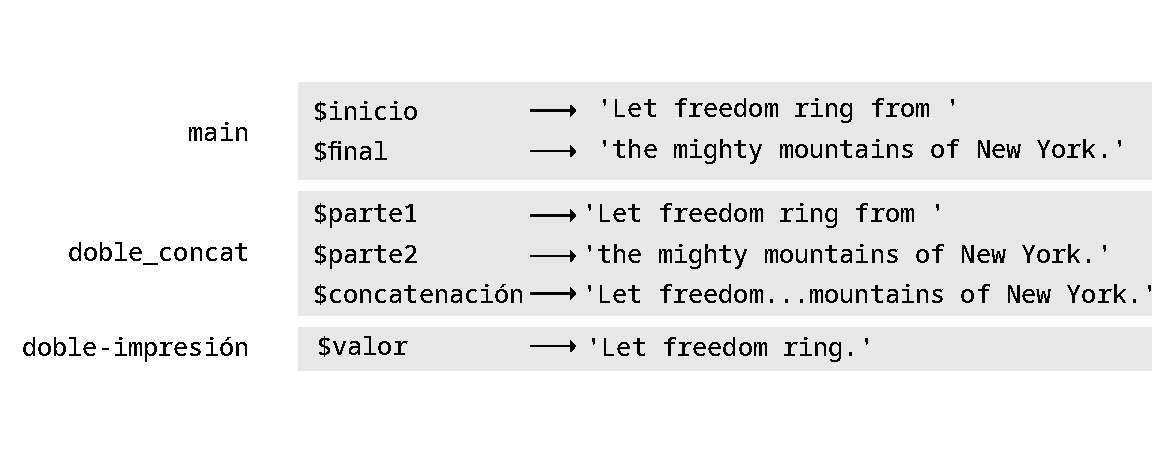
\includegraphics[scale=0.8]{figs/stack_diagram.pdf}}
%{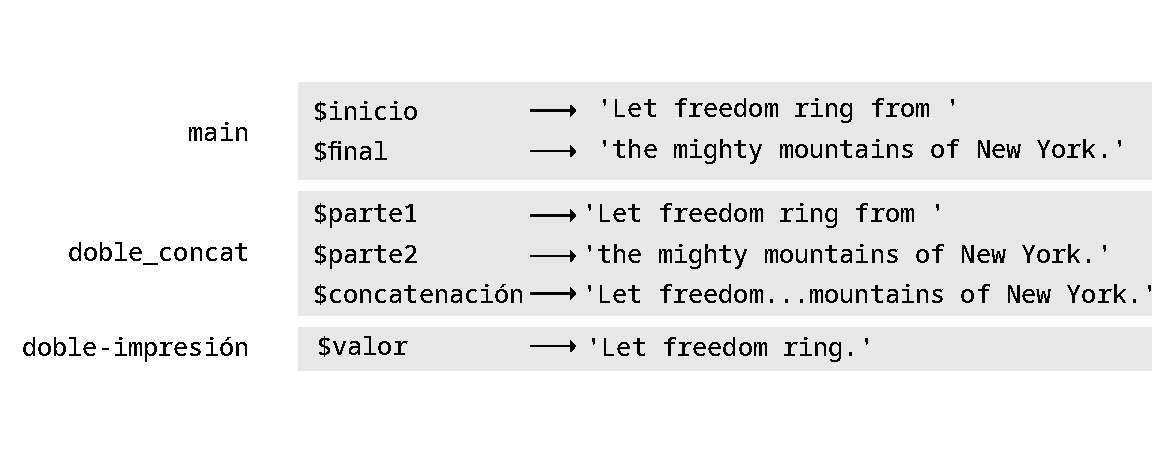
\includegraphics[scale=1.2]{figs/stack_diagram.png}}
\caption{Diagrama de estado.}
\label{fig.stack}
\end{figure}

Los marcos están organizados en la pila para indicar cual función
llama a cual. En este ejemplo, \verb|doble-impresión| fue llamada
por \verb|doble_concat|, y \verb|doble_concat| fue llamada por 
\verb|main|, el cual es un nombre especial para el marco superior.
Cuando creas una variable fuera de cualquier función, dicha variable
le pertenece a \verb|main|.

Cada parámetro hace referencia al mismo valor que su argumento correspondiente.
Así que, {\tt \$parte1} tiene el mismo valor que {\tt \$inicio},
{\tt \$parte2} tiene el mismo valor que {\tt \$final} y {\tt \$valor}
tiene el mismo valor que {\tt \$concatenación}.



\section{Funciones Fructuosas y Funciones Voids}
\index{fruitful function}
\index{void function}
\index{function, fruitful}
\index{function, void} 

Algunas de las funciones que hemos usados, tal como las 
funciones matemáticas, devuelven resultados y son útiles
en cuanto podamos usar el valor devuelto; por falta de un 
mejor nombre, las podamos llamar {\bf funciones fructuosas}.
Otras funciones, tal como \verb|doble-impresión|, realizan una
acción pero no parecen devolver un valor (aunque en verdad devuelve
un valor, {\tt True}, pero no estamos interesados en este valor).
Estas funciones son algunas veces llamadas funciones vacías o funciones
void en otros lenguajes de programación.

En algunos lenguajes de programación, tales como Pascal o Ada,
existe una gran distinción entre una \emph{función} (la cual
devuelve un valor) y un \emph{procedimiento} (el cual no devuelve
ningún valor); ellas son definidas con diferentes palabras claves.
Dicha distinción no aplica en Perl y en la mayoría de los 
lenguajes de programación modernos.

De hecho, desde un punto de vista sintáctico, las funciones de Perl
siempre devuelven un valor. Así que la distinción entre una función
``fructuosa`` y ``void`` no existe sintáctica, solo semánticamente, i.e.,
desde el punto de vista del significado del programa: tal vez necesitamos
usar el valor devuelto, o tal vez no.

Otra distinción que se hace comúnmente entre funciones y mutadores es
que las funciones no cambian el estado inicial de los argumentos 
que se les pasa mientras que los mutadores modifican los argumentos. 
No usaremos esta distinción aquí, pero es útil mantenerla presente.

Cuando llamas una función fructuosa, es muy común que quieras
hacer algo con el resultado; por ejemplo, podrías asignarlo a una
variable o usarlo como parte de una expresión:
 
\begin{verbatim}
my $altura = sin $radianes;
my $aúreo = (sqrt(5) + 1) / 2;
\end{verbatim}
%
Cuando llamas una función en el modo interactivo (en
el REPL), Perl usualmente muestra el resultado inmediatamente:

\begin{verbatim}
> sqrt 5;
2.23606797749979
\end{verbatim}
%
¡Pero en un script, si llamas una función fructuosa por sí misma,
el valor de retorno se pierde para siempre! En algunos casos, el 
compilador será capaz de advertirte, pero no siempre. Por ejemplo,
considera el siguiente programa:

\begin{verbatim}
my $cinco = 5;
sqrt $cinco;
say $cinco;
\end{verbatim}

Este ejemplo produce la siguiente advertencia:

\begin{verbatim}
WARNINGS for /home/Laurent/perl6_tests/sqrt.pl6:
Useless use of "sqrt $cinco" in expression "sqrt $cinco" in sink context (line 2)
5
\end{verbatim}
%
El script computa la raíz cuadrada de 5, pero 
dado que no almacena o muestra el resultado, no es muy útil.
\index{interactive mode}
\index{script mode}

Funciones void muestran algo en la pantalla, guardan algún dato
en un archivo, modifican una variable o un objeto, o tienen
algún otro efecto, pero generalmente no tienen un valor de
retorno, o por lo menos algo no muy útil. Si asignas el resultado
a una variable, puedes conseguir el valor de retorno de la subrutina,
el valor de la última expresión que fue evaluada en la función,
o un valor especial tal como {\tt Any}, el cual esencialmente se
refiere a algo que no ha sido definido, o {\tt Nil}.
\index{Any special value}
\index{special value!Any}
%

Las subrutinas que hemos escrito hasta ahora esencialmente muestran cosas
en la pantalla. En ese caso, ellas devuelven {\tt True}, por lo
menos cuando la impresión fue exitoso. Aunque ellas devuelven un 
valor verdadero, lo que ellas devuelven no es muy útil y podemos
considerarlas funciones void para nuestro propósitos.

El siguiente es un ejemplo de una subrutina fructuosa bien simple:
\index{return}

\begin{verbatim}
> sub cuadrado($número) { return $número ** 2 }
sub cuadrado ($número) { #`(Sub|118134416) ... }
> say cuadrado 5;
25
\end{verbatim}

El mensaje \verb'Sub|118134416' mostrado por el REPL
es solo un identificador interno de la subrutina que hemos
definido.

La sentencia {\tt return} le indica a la función que termine
la ejecución de la función en esta sentencia y devuelva el valor 
de la siguiente expresión a donde fue llamada. En tal caso 
donde el programa está ejecutando la última sentencia de una 
función, la palabra clave return puede ser omitida dado que la
función devolverá el valor de la última sentencia evaluada,
así que la subrutina {\tt cuadrado} podría ser escrita de 
la siguiente manera:
\begin{verbatim}
sub cuadrado($número) { 
    $número ** 2 
}
\end{verbatim}

Usaremos funciones fructuosas más extensivamente en los 
siguientes capítulos.

\section{Signaturas de Funciones}
\index{function!signature}
\index{signature}

Cuando una función recibe argumentos, los cuales son
almacenados en los parámetros, la parte de la definición
de función que describe los parámetros entre los 
paréntesis se llama la {\bf signatura de la función}. Las 
signaturas de funciones que hemos visto hasta ahora son bien 
simple y consisten de un solo parámetro o posiblemente
una lista de parámetros.

Las signaturas pueden proveer una plétora de información
sobre los parámetros usados por la función. Primero, puedes
definir el tipo de los parámetros. Algunas funciones hacen 
sentido solo si sus parámetros son numéricos y deberían
probablemente levantar un error si ellas reciben una
cadena de texto que no pueden ser convertida a un valor
numérico. Por ejemplo, si defines una función {\tt mitad}
que computa el valor igual a su argumento divido por 2,
no hace sentido tratar de computar la mitad de una
cadena de texto que no es numérica. Dicha función
podría escribirse así:
\index{type!parameter}
\index{parameter type}

\begin{verbatim}
sub mitad(Int $número) { 
    return $número / 2 
}
say mitad 84; # -> 42
\end{verbatim}

Si está función es llamada con una cadena de texto,
conseguimos el siguiente error:
\index{type!String}

\begin{verbatim}
> say mitad "Douglas Adams"
===SORRY!=== Error while compiling <unknown file>
Calling mitad(Str) will never work with declared signature (Int $number)
at <unknown file>:1
------> say <HERE>mitad "Douglas Adams"
\end{verbatim}

El tipo {\tt Int} incluido en la signatura de la función es
una restricción de tipo que puede ayudar a prevenir errores
sutiles. En algunos casos, también pueden ser una molestia.
Considera el fragmento de código:
\index{constraint!type}
\index{type!constraint}
\index{type!Int}
\index{signature}


\begin{verbatim}
sub mitad(Int $número) {  $número / 2 }
say mitad "84"; # -> ERROR
\end{verbatim}

Dado que el argumento de la subrutina {\tt mitad} es {\tt "84"},
i.e., una cadena de texto, este código fallará con un error de 
tipo. Si no hubiésemos incluidos el tipo {\tt Int} en la signatura,
el script habría convertido (o \emph{coaccionado}) la cadena de
texto "84" en un número, dividido por 2, y mostrado el
resultado esperado:
\index{type!String}
\index{type!coercion}
\index{coercion!type}

\begin{verbatim}
sub mitad($número) { $número / 2 }
say mitad "84"; # -> 42
\end{verbatim}

En algunos casos, tu quieres que esta conversión ocurra,
en otras, no quieres. Es tu deber decidir si quieres
tipado estricto o no, dependiendo en la
situación específica y necesidad. Es probablemente útil usar 
tipos en los parámetros en muchos casos, pero puede 
volverse un obstáculo en algunas situaciones. Perl~6 te deja 
decidir qué tan estricto deseas ser sobre estas cosas.

Nuestra subrutina original {\tt mitad} tiene otra limitación: 
solo funciona con números enteros. Pero una función que 
devuelve la mitad de su argumento debería supuestamente
ser útil para números racionales o hasta otros números. 
Puedes usar los tipos {\tt Real}  o {\tt Numeric} para
hacer la función más general (la diferencia entre los
tipos  es que el tipo {Numeric} aceptará no solo números
{\tt Real}es pero también números complejos ({\tt Complex})
\footnote{~Los números complejos son un concepto matemático
poderoso. Ellos son números de la forma $a + bi$, donde 
$a$ y $b$ son un números reales y $i$ es un número imaginario
de tal modo que $i²$ es igual a $-1$.}). Como sucede con
números complejos, el elegir un tipo {\tt Numeric} abre más 
posibilidades:
\index{Numeric type}
\index{type!Numeric}
\index{Real type}
\index{type!Real}
\index{Complex type}
\index{type!Complex}
\index{type!Int}

\begin{verbatim}
sub mitad(Numeric $número) { $número / 2 }
say mitad(3+4i); # -> 1.5+2i
\end{verbatim}

La siguiente tabla resume e ilustra  algunos de los varios
tipos que hemos visto hasta ahora.

\begin{center}
\begin{tabular}{|l|c|}  \hline
\label{types}
\emph{Tipo} & \emph{Ejemplo}   \\ \hline
String      & \verb'"Una cadena de texto (string)"', \verb"'Hola'", \verb'"42"' \\ \hline
Integer     & \verb' -3, -2, 0, 2, 42' \\ \hline
Rational    & \verb' 1/2, 0.5, 3,14159, 22/7, 42.0' \\ \hline
Real        & $\pi$, pi, $\surd{2}$, \emph{e}, $\log 42$, $\sin 0.7$\\ \hline
Complex     & $5.4 + 3i$ \\ \hline
\end{tabular}
\end{center}
\index{String type}
\index{type!String}


\section{Parámetros Inmutables y Mutables}

\index{immutable parameter}
\index{mutable parameter}
\index{parameter!mutable}
\index{parameter!immutable}
Por defecto, los parámetros de una subrutina son apodos {\bf inmutables}
para los argumentos pasados a la subrutina. En otras palabras,
ellos no pueden ser cambiados dentro de la función y tú no puedes
modificar el argumento accidentalmente donde la función es llamada:

\begin{verbatim}
sub más-tres(Int $número) { $número += 3}
my $valor = 5;
say más-tres $valor; # ERROR: Cannot assign to an immutable value
\end{verbatim}

En algunos otros lenguajes, este comportamiento es conocido
como una ``llamada por valor``: en términos generales, 
la subrutina recibe (por defecto) un valor y no una variable, y 
el parámetro por lo tanto no puede ser modificado.
\index{call by reference}

Si quieres cambiar el valor del parámetro dentro de la subrutina
(pero sin cambiar el argumento), tú puedes agregar el \emph{trait} 
{\tt is copy} a la signatura:
\index{signature}
\index{trait}
\index{is copy trait}
\index{trait!is copy}

\begin{verbatim}
sub más-tres(Int $número is copy) { $número += 3}
my $valor = 5;
say más-tres $valor;  # 8
say $valor;             # 5 (valor de la variable intacto)
\end{verbatim}
%
Un {\bf trait} (rasgo) es una propiedad del parámetro definida
al tiempo de compilación. Aquí, el parámetro {\tt \$número} es
modificado dentro de la subrutina y el valor incrementado es devuelto e 
imprimido como 8, pero, dentro de la función que hace la llamada,
la variable usada como un argumento para la función, {\tt \$valor},
no es modificada (es todavía 5).

Aunque esto puede ser algunas veces peligroso, tú puedes 
también querer escribir una subrutina que modifica su argumento
en el lugar donde la función es llamada. Para esto, puedes usar
el \emph{trait} {\tt is rw} en la signatura:
\index{is rw trait}
\index{trait!is rw}

\begin{verbatim}
sub más-tres(Int $número is rw) { $número += 3}
my $valor = 5;
say más-tres $valor;  # 8
say $valor;             # 8 ($valor es modificada)
\end{verbatim}
%
Con el trait {\tt is rw}, el parámetro {\tt \$número} está ahora
\emph{vinculado} al argumento {\tt \$valor}, así que cualquier
cambio hecho al usar {\tt \$número} dentro de la subrutina será 
inmediatamente aplicado a {\tt \$valor} en lugar donde la función
es llamada,porque {\tt \$número} y {\tt \$valor} son solo nombres
diferentes para la misma cosa (ambos hacen referencia a la misma
dirección de memoria). El argumento es ahora totalmente \emph{mutable}.

En algunos otros lenguajes de programación, esto se conoce como
``llamada por referencia``, porque, en aquellos lenguajes, 
si tu pasas una referencia (o un puntero) de una variable a una
función, entonces es posible que la función pueda modificar la
variable referida por la referencia.
\index{call by reference}


\section{Funciones y Subrutinas: Ciudadanos de Primera Clase}
\index{first-class object}
\index{object, first-class}
\index{function!higher-order}
\label{first_class}

Las subrutinas y otros objetos de código se pueden pasar como 
los valores, como cualquier variable, literal u objeto. Entonces
se dice que las funciones son {\bf objetos de primera clase} o algunas
veces, ciudadanos de primera clase o funciones de orden superior. 
Esto significa que una función de Perl (no el valor que devuelve sino
su código) es un valor que puedes asignar a una variable o pasarlo como
un argumento. Por ejemplo, \verb|do-twice| es una subrutina que toma
una función como argumento y la llama dos veces:

\begin{verbatim}
sub do-twice($código) {
    $código(); 
    $código();
}
\end{verbatim}

Aquí, el parámetro \verb|$código| se refiere a una función o cualquier
otro objeto que se pueda llamar. Esto es un ejemplo que usa \verb|do-twice|
para llamar una función llamada \verb|saludar| dos veces:

\begin{verbatim}
sub saludar {
    say "¡Hola Mundo!";
}
do-twice &saludar;
\end{verbatim}

Esto imprimirá:
\begin{verbatim}
¡Hola Mundo!
¡Hola Mundo!
\end{verbatim}

El sigilo \verb|&| se coloca antes del nombre de la subrutina 
en la lista de argumentos para dejarle saber a Perl que estás
pasando una subrutina o cualquier objeto de código 
que se puede llamar (y no estás llamando la
subrutina en el momento).
\index{sigil}
\index{ampersand sigil}
%\index{$&$ sigil}
%\index{sigil!$&$}

De hecho, sería más idiomático usar también el sigilo \verb|&|
en la definición de la subrutina \verb|do-twice| para especificar
que el parámetro es un objeto de código que se puede llamar:
\index{idiomatic}

\begin{verbatim}
sub do-twice(&código) {
    &código(); 
    &código();
}
\end{verbatim}

De igual manera:
\begin{verbatim}
sub do-twice(&código) {
    código(); 
    código();
}
\end{verbatim}

La sintaxis con el sigilo \verb|&| tiene el beneficio de
proveer un mejor mensaje de error si cometes un error y le pasas
a \verb|do-twice| algo que no se puede llamar. 

Todas las funciones que hemos vistos hasta ahora han tenido nombre,
pero no es necesario que una función tenga un nombre y por lo tanto,
puede ser una función {\bf anónima}. Por ejemplo, 
se puede almacenar directamente en una variable escalar:
\index{anonymous function}
\index{function!anonymous}

\begin{verbatim}
my $saludar = sub {
    say "¡Hola Mundo!";
};
$saludar();               # imprime "¡Hola Mundo!"
do-twice $saludar;        # imprime "¡Hola Mundo!" dos veces
\end{verbatim}

Se podría argumentar que la subrutina \verb|$saludar| no es realmente
anónima, debido a que está almacenada en una variable escalar 
que podría de alguna manera ser considerada su nombre. Pero realmente
la subrutina no posee un nombre; solo sucede que está asignada a una
variable escalar. Para demostrar que la subrutina no tiene nombre 
alguno, considera lo siguiente:

\begin{verbatim}
do-twice(sub {say "¡Hola Mundo!"} );
\end{verbatim}

Esto imprimirá "¡Hola Mundo!" sin ningún problema. Si la función
\verb|do-twice| se ha declarado posteriormente, puedes hasta 
simplificar la sintaxis y omitir los paréntesis:

\begin{verbatim}
do-twice sub {say "¡Hola Mundo!"};
\end{verbatim}

Para casos simples donde no hay necesidad de pasar un argumento
o devolver un valor, puedes omitir la palabra clave \verb|sub|
y pasar un bloque de código directamente a la función:
\index{code block}

\begin{verbatim}
do-twice {say "¡Hola Mundo!"};
do-twice {say "¡Buen día!"};
\end{verbatim}

Como puedes observar, \verb|do-twice| es una subrutina \emph{genérica}
cuyo trabajo es ejecutar dos veces cualquier función o bloque
de código que se le pasa, sin ningún conocimiento sobre lo que la 
función o el bloque de código hace. Este es un concepto poderoso
usado en algunas técnicas de programación avanzadas que discutiremos
más adelante.
\index{generic subroutine}

Las subrutinas se pueden también pasar como valores de
retorno desde otras subrutinas:
\index{factory, function}
\index{function!factory}

\begin{verbatim}
> sub crear-función ($persona) { return sub { say "¡Hola $persona!"}}
# Crear dos funciones de saludos
sub crear-función ($persona) { #`(Sub|176738440) ... }
> my $saludar_mundo = crear-función "Mundo";
sub () { #`(Sub|176738592) ... }
> my $saludar_amigo = crear-función "querido amigo";
sub () { #`(Sub|176739048) ... }
# Usar las funciones de saludos
> $saludar_mundo();
¡Hola Mundo!
> $saludar_amigo();
¡Hola querido amigo!
\end{verbatim} 

Aquí, la función \verb|crear-función| devuelve una subrutina que saluda
a alguien. Se llama dos veces con dos argumentos diferentes para crear
dos funciones diferentes al tiempo de ejecución, \verb|$saludar_mundo|
y \verb|$saludar_amigo|. Una función como \verb|crear-función| es algunas
veces conocida como una \emph{factoría de funciones} porque puedes crear 
un número determinado de funciones con solo llamar a \verb|crear-función|. Este 
ejemplo puede parecer una manera complicada de hacer algo tan simple. 
Lo que pasa es que en este momento es muy prematuro dar ejemplos útiles,
no obstante esta es una técnica de programación muy poderosa.

Regresaremos a estas técnicas a lo largo de este libro y hasta dedicaremos
un capítulo entero (capítulo~\ref{functional programming}) 
para este asunto y otros temas relacionados.


\section{¿Por qué Funciones y Subrutinas?}
\index{function, reasons for}

Debido a que no está claro el por qué de dividir un programa
en funciones o subrutinas, aquí discutimos varias razones:

\begin{itemize}

\item La creación de una subrutina nueva te da la oportunidad
de nombrar un grupo de sentencias, lo cual hace tu programa más
fácil de leer y depurar. Las subrutinas también ayudan a hacer el 
flujo de ejecución más claro para el lector.

\item Las subrutinas pueden reducir el tamaño de un programa
al eliminar código repetitivo. Más adelante, si haces un cambio,
solamente tienes que hacerlo en un solo lugar.
\index{code repetition}

\item La división de un programa largo en subrutinas te permite
depurar las partes una a una y después ensamblarlas en un todo
que funciona.

\item Las subrutinas que son bien diseñadas usualmente son 
útiles para muchos programas. Una vez que escribes y depuras una,
la puedes reusar.
\index{code reuse}
\index{abstraction}

\item La creación de subrutinas es una de las maneras más
útiles de descomponer un problema difícil en tareas pequeñas 
más fáciles y de crear capas sucesivas de abstracción, las cuales
son las llaves para resolver problemas complejos.
\index{abstraction}

\index{black box}
\item Escribir buenas subrutinas te permite crear cajas negras,
con una entrada y una salida conocida. Así que no tienes que pensar
sobre ellas cuando trabajas en algo más. Se han convertido en
herramientas. Una vez que ensamblas un taladro, no necesitas 
pensar sobre cómo trabaja internamente cuando lo usas para construir
o reparar algo.
\index{black box}

\item En el mundo actual de código abierto, existe la oportunidad
que tu código tendrá que ser comprendido, mantenido or mejorado por 
otras personas. La programación se ha vuelto más y más una actividad
social y la descomposición de tu código en pequeñas subrutinas cuyo
propósito es fácil de entender hará el trabajo de las otras personas
más fácil. Y tú estarás más deleitado cuando la persona que tenga
que mantener o refactorizar tu código sea... tú.  
\index{open source code}

\end{itemize}


\section{Depuración de Programas}

Una de las más importantes habilidades de programación 
que tú adquirirás es la depuración. Aunque algunas veces 
puede ser frustrante, la depuración es una de las partes más
intelectualmente rica, estimulante e interesante de la
programación.  
\index{experimental debugging}
\index{debugging!experimental}

En alguna forma, la depuración se parece al trabajo detectivesco.
Eres confrontado con pistas y debes inferir los procesos y eventos
que conllevaron a los resultados que ves.

La depuración es como una ciencia experimental. Una vez que tienes
una idea de lo que no funciona, modificas el programa e intentas 
nuevamente. Si la hipótesis era correcta, puedes predecir el resultado
de la modificación, y te acercas más a un programa que funciona. Si la
hipótesis era incorrecta, tienes que producir una nueva hipótesis. 
Como Sherlock Holmes señaló, 


Debugging is also like an experimental science.  Once you have an idea
about what is going wrong, you modify your program and try again.  If
your hypothesis was correct, you can predict the result of the
modification, and you take a step closer to a working program.  If
your hypothesis was wrong, you have to come up with a new one.  As
Sherlock Holmes pointed out, ``Cuando todo aquello que es imposible 
ha sido eliminado, lo que quede, por muy improbable que parezca, 
es la verdad``
(A. Conan Doyle, {\em El signo de los cuatro}).
\index{Holmes, Sherlock}
\index{Conan Doyle, Arthur}

En los casos donde no eres capaz de producir una hipótesis
sobre lo que no funciona, puedes intentar introducir
código del cual espera un determinado tipo de error, 
una ``hipótesis negativa``. Algunas veces puedes aprender 
mucho del hecho de que no creó el error que se esperaba. 
Crear una hipótesis no significa necesariamente que tienes 
una idea sobre cómo hacerlo funcionar, también podría ser
una hipótesis sobre cómo hacerlo fallar.

Para algunas personas, la programación y la depuración son
la misma cosa. Es decir, la programación es el proceso de 
depurar gradualmente un programa hasta que hace lo que quieres.
La idea es que tú deberías comenzar con un programa que funciona y 
hacer pequeñas modificaciones, y depurarlas según avanzas.

Por ejemplo, Linux es un sistema operativo que contiene millones 
de líneas de código. Sin embargo, todo comenzó con un simple programa
que Linus Torvalds usó para explorar el chip Intel 80386. De acuerdo
a Larry Greenfield, "Uno de los proyectos iniciales de Linus fue un 
programa que cambiaba entre la impresión de \verb|AAAA| y \verb|BBBB|.
Luego éste evolucionó en Linux.``
({\em The Linux Users' Guide} Beta Version 1).
\index{Linux}


\section{Glosario}

\begin{description}

\item[Función] Una secuencia de sentencias que realiza 
una función útil. Las funciones pueden cero o más argumentos
y pueden producir o no producir un resultado. Perl viene con 
muchas funciones integradas, y tú puedes crear tus propias
funciones. En Perl, las funciones definidas por el usuario son
usualmente conocidas como subrutinas.
\index{function}

\item[Definición de una función]  Una sentencia que crea una función
nueva, especifica su nombre, sus parámetros, y las sentencias
que contiene.
\index{function!definition}

\item[Cabecera] La primera línea de la definición de la 
función.
\index{header}

\item[Cuerpo] La secuencia de sentencias dentro de la definición
de la función, usualmente en un bloque de código delimitado por
llaves.
\index{body}

\item[Parámetro] Un nombre que usa dentro de la subrutina
para referirse al valor que se pasa como un argumento.
\index{parameter}

\item[Llamada de función] Una sentencia que ejecuta la función.
Consiste del nombre de la función seguido por una lista de 
argumentos, la cual puede o no puede estar encerrada por
paréntesis.
\index{function!call}

\item[Argumento] Una valor que se provee a la función cuando
ésta se llama. Este valor es asignado al parámetro 
correspondiente en la función.
\index{argument}

\item[Variable lexical] Una variable definida dentro de una
subrutina o un bloque de código. Una variable lexical definida
dentro de una función se puede usar solo dentro de la función.
\index{local variable}

\item[Valor de retorno]  El resultado de una función. Si una llamada
de función se usa como una expresión, el valor de retorno es el valor 
de la expresión.
\index{return!value}

\item[Any]  Una valor especial típicamente encontrado en 
las variables a las cuales no se le ha asignado un valor. Es 
también un valor especial devuelto por algunas funciones que 
llamamos ``void`` (porque ellas devuelven algo que no es
generalmente útil tal como ``Any``).
\index{Any special value}
\index{special value!Any}

\item[Nil] Tambié un valor especial devuelto algunas veces
 por las subrutinas ``void``.

\item[Módulo] Una archivo que contiene una colección
de funciones relacionadas y otras definiciones.
\index{module}

\item[Sentencia use] Una sentencia que lee un módulo y 
usualmente exporta algunas funciones.
\index{use statement}
\index{statement!use}

\item[Composición] Usar una expresión como parte de
una expresión más compleja o una sentencia como parte
de una sentencia más larga.
\index{composition}

\item[Flujo de ejecución]  El orden en cual las sentencias
son ejecutadas.
\index{flow of execution}

\item[Diagrama de pila]  Una representación gráfica de una
pila de subrutinas, sus variables, y los valores a los cuales
hacen referencia.
\index{stack diagram}

\item[Marco]  Una caja en un diagrama de pila que representa una
llamada de subrutina. Contiene las variables locales y los 
parámetros de la subrutina.
\index{function!frame}
\index{frame}

\item[Función fructuosa] Una functión que devuelve un valor
útil.
\index{fruitful function}

\item[Funcción void] Una función o subrutina que no devuelve
un valor útil.
\index{void function}

\item[Signatura de una función] La parte de la definición de 
una función (usualmente entre paréntesis) que define 
sus parámetros y posiblemente sus tipos y otras propiedades.
\index{function!signature}
\index{signature}

\item[Parámetros inmutables] Una parámetro de una función
o subrutina que no se puede cambiar dentro del cuerpo de
la función. Por defecto, los parámetros de una
subrutinas son inmutables.
\index{immutable parameter}

\item[Trait] Una propiedad de un parámetro de una función
o subrutina que es definido al tiempo de compilación.
\index{trait}

\item[Objeto de primera clase] Las subrutinas de Perl se
dice que son objetos de orden superior o objetos de primera 
clase porque ellas se pueden pasar como argumentos a 
otras subrutinas o como valores de retorno, como cualquier
otro objeto.
\index{first-class object}
\index{object, first-class}

\item[Función anónima] Una función que no tiene nombre.
\index{anonymous function}
\index{function!anonymous}

\item[Factoría de funciones] Una función de produce otras 
funciones como valores de retorno.
\index{factory, function}
\index{function!factory}

\end{description}


\section{Ejercicios}

\begin{exercise}
\index{chars function}
\index{function!chars}
\label{right_justify}

Escribe una subrutina llamada \verb|alinear-a-derecha| 
que toma una cadena de texto llamada {\tt \$cadena-entrada}
como parámetro e imprime la cadena de texto con suficiente
espacio blanco de tal modo que la última letra de la cadena
de texto esté en la columna 70 de la pantalla.

\begin{verbatim}[fontshape=up]
> alinear-a-derecha('Larry Wall')
                                                           Larry Wall
\end{verbatim}

Pista: Usa la concatenación de cadena de texto y repetición. 
De igual manera, Perl provee una función integrada llamada 
{\tt chars} que devuelve la longitud de una cadena, así que
el valor de \verb"chars 'Larry Wall'" or \verb"'Larry Wall'.chars"
es 10. Solución: \ref{sol_right_justify}.

\end{exercise}


\begin{exercise}
\index{first-class object}
\index{object!first-class}
\index{do-twice}
\label{do_it_twice}

Hemos visto que las funciones y otros objetos de código 
se pueden pasar como valores, tal como cualquier objeto. Se dice
que las funciones \emph{objetos de primera clase}. Por ejemplo, 
\verb|do-twice| es una función que toma una función como un
argumento y la llama dos veces:

\begin{verbatim}[fontshape=up]
sub do-twice($código) {
    $código(); 
    $código();
}
sub saludar {
    say "Hello World!";
}
do-twice(&saludar);
\end{verbatim}

\begin{enumerate}

\item Escribe este ejemplo en un script y 
pruébalo.

\item Modifica la función \verb|do-twice| para que tome
dos argumentos, una función y un valor, y llama la función
dos veces, pasando el valor como una argumento.

\item Copia la definición de \verb|doble-impresión| del 
inicio de este capítulo en tu script.

\item Usa la versión modificada de \verb|do-twice| para llamar
a \verb|doble-impresión| dos veces, pasando como argumento
la cadena de texto ``What's up doc''.

\item Define una función nueva llamada \verb|do-four|
que toma una función y un valor y llama la función
cuatro veces, pasando el valor como un argumento. Deberían
haber solo dos sentencias en el cuerpo de la función, no cuatro.

\end{enumerate}

Solución: \ref{sol_do_it_twice}.

\end{exercise}



\begin{exercise}
\label{draw_a_grid}
\index{print-grid}

Nota: Debes resolver este ejercicio con solo el uso de
las sentencias y otras características que hemos
discutidos hasta ahora.

\begin{enumerate}

\item Escribe una subrutina que dibuje una cuadrícula como 
la siguiente:
\index{grid}

\begin{verbatim}[fontshape=up]
+ - - - - + - - - - +
|         |         |
|         |         |
|         |         |
|         |         |
+ - - - - + - - - - +
|         |         |
|         |         |
|         |         |
|         |         |
+ - - - - + - - - - +
\end{verbatim}
%
Pista: para imprimir más de un valor en una línea, puedes
imprimir una secuencia de valores separados por coma:

\begin{verbatim}[fontshape=up]
  say '+', '-';
\end{verbatim}
%
La función {\tt say} imprime sus argumentis con una nueva línea
al final (la cual avanza el cursor a la siguiente línea). Si no
quieres colocar el cursor en la siguiente línea, entonces usa
la función {\tt print}:

\begin{verbatim}[fontshape=up]
  print '+', ' ';
  print '-';
\end{verbatim}
%
La salida de estas sentencias es ``+ -''.

Una sentencia {\tt say} con una cadena de texto vacía como
argumento termina la actual línea y va a la siguiente
línea.

\item Escribe una subrutina que dibuje una cuadrícula similar con
cuatro filas y cuatro columnas.

\end{enumerate}

Solución: \ref{sol_draw_a_grid}
\index{print-grid}.

Crédito: Este ejercicio está basado en un ejercicio en Oualline, {\em
    Practical C Programming, Third Edition}, O'Reilly Media, 1997.

\end{exercise}

